\section{Sensors}
To acquire relevant data from the golf course, and to enable processing of this data in a digital domain, there has to be sensors. The sensors must be capable of gathering data, and returning a value, either as a digital or analog signal than can be processed by a computation unit. As multiple sensors are needed, the price point is considered relevant, as it will cause the overall cost of the solution to grow.

Prices mentioned in this section is based on results of online searches, and might be different at the time of reading this. They don't serve to make accurate calculations, but rather to get a general idea of the expenses required to include them in a solution.

\subsection{Moisture Sensor}
To obtain information about the moisture of soil on the gold course, a moisture sensor is needed. The moisture can change relatively quickly depending on rain and and type of soil. Sensors for monitoring moisture can be acquired for prices at about 1\$.%Simple moisture sensors are build as a pair of spikes inserted in the ground\todo{MAJOR generalization without source}. Between them a current is being sent, and the resistance of the ground is measured. Based on this value the moisture can be calculated. %INSERTNAMEHERE\todo{find navnet -.-, og find documentation, er ebays beskrivelse gyldig?} .

\begin{figure}[H]
\centering
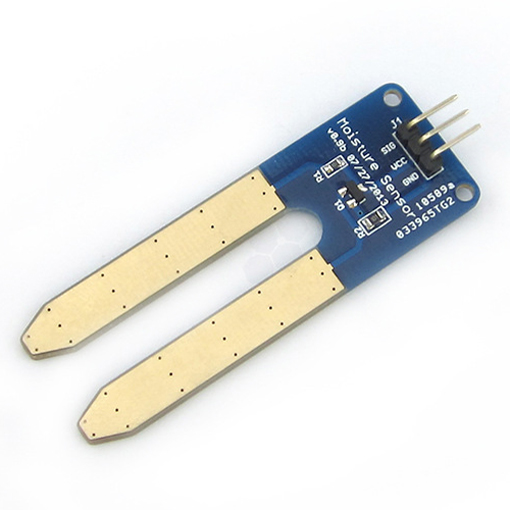
\includegraphics[width=0.6\textwidth]{chapters/analysis/figs/soilMoistureSensor.jpg}
\caption{Soil moisture sensor.}
\label{fig:moistureSensor}
\end{figure}

\subsection{Soil pH Sensor} \todo{the more i look, the harder it seem to prove this even exists.}
To get information about the acidity or alkalinity of the soil, a pH is needed. These, however, are both expensive and can be arguably inaccurate, so they will not be covered in depth, as they fall shot of our problem. 

\begin{figure}[H]
\centering
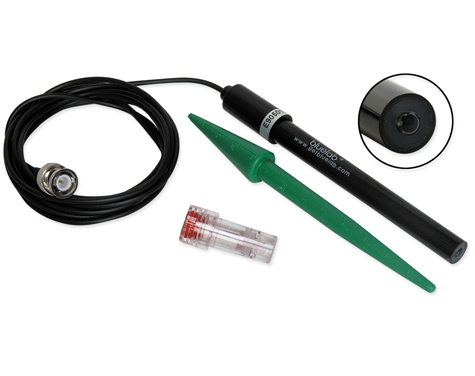
\includegraphics[width=0.6\textwidth]{chapters/analysis/figs/soilPhProbe.jpg}
\caption{Soil pH sensor with probe.}
\label{fig:phSensor}
\end{figure}

\subsection{Soil Compaction Sensor}
To get information about the compaction of the ground, a sensor for measuring this can be helpful. %However this is not data that changes as rapidly as moisture and pH\todo{source - and convincing?}. The slow data changes and 
The price point of the sensors, which at time of writing is found on listings from 200\$ makes this less interesting when considering the amount of needed sensors. % in discarding this sensor from further analysis.

\todo{Jeg ville mene det måske var en idé at fjerne Compaction og ph sensors helt og så skrive mere on Moisture sensors. - Få sensor test med i dette afsnit}